\documentclass[aspectratio=169]{beamer}
\usepackage{fontspec}
\usepackage[vietnamese]{babel}
\usepackage{graphicx}
\usepackage{booktabs}
\usepackage{listings}
\usepackage{caption}

% Cài đặt theme
\usetheme{Madrid}
\usecolortheme{default}
\setbeamertemplate{navigation symbols}{}
\setbeamertemplate{caption}[numbered]
\setbeamertemplate{footline}[frame number]

% Cấu hình listings cho code Python
\lstset{
    language=Python,
    basicstyle=\ttfamily\scriptsize,
    keywordstyle=\color{blue},
    stringstyle=\color{red},
    commentstyle=\color{green!60!black},
    numbers=left,
    numberstyle=\tiny\color{gray},
    stepnumber=1,
    showstringspaces=false,
    tabsize=4,
    breaklines=true,
    breakatwhitespace=true,
    frame=single,
    backgroundcolor=\color{gray!10}
}

\title[Chương 15: RNN \& CNN cho Chuỗi]{Chương 15: Xử lý Chuỗi bằng RNN và CNN}
\author[Giảng viên]{Giảng viên: [Tên Giảng Viên]}
\institute[Đại Học Đông Á]{Đại Học Đông Á}
\date{\today}

\begin{document}

\begin{frame}
    \titlepage
\end{frame}

\begin{frame}{Nội dung Chương 15}
    \tableofcontents
\end{frame}

\section{1. Dữ liệu Chuỗi và Mạng nơ-ron hồi quy (RNN)}

\begin{frame}{Khái niệm: Dữ liệu Chuỗi (Sequence Data) là gì?}
    \begin{itemize}
        \item Trong các chương trước, chúng ta xử lý dữ liệu nơi mỗi điểm dữ liệu là \textbf{độc lập và phân phối chuẩn (i.i.d)}.
        \item Tuy nhiên, trong \textbf{dữ liệu chuỗi}, tính thứ tự và sự phụ thuộc thời gian là cốt lõi.
        \item Ví dụ điển hình:
        \begin{itemize}
            \item \textit{Chuỗi thời gian kinh tế:} Giá cổ phiếu qua các ngày, GDP hằng năm.
            \item \textit{Dữ liệu y tế:} Điện tâm đồ (ECG), điện não đồ (EEG).
            \item \textit{Ngôn ngữ tự nhiên (NLP):} Một câu là một chuỗi các từ có cấu trúc ngữ pháp.
            \item \textit{Âm thanh / Video:} Chuỗi các khung hình và sóng âm theo thời gian.
        \end{itemize}
    \end{itemize}
\end{frame}

\begin{frame}{Giới hạn của Mạng Truyền thẳng (Feedforward Networks)}
    \begin{itemize}
        \item \textbf{Mạng truyền thẳng (như MLP, CNN truyền thống)}:
        \begin{itemize}
            \item Kích thước đầu vào bị cố định (Fixed-size input).
            \item Không có bộ nhớ (Memoryless): Mỗi lần nhận đầu vào mới, mạng quên hoàn toàn các đầu vào trước đó.
            \item Không nắm bắt được phụ thuộc xa (Long-term dependencies) trừ khi nạp một lượng lớn đầu vào cùng lúc.
        \end{itemize}
        \item Giải pháp: Cần một mạng có khả năng \textbf{lưu giữ trạng thái} của những gì nó đã thấy.
    \end{itemize}
\end{frame}

\begin{frame}{Kiến trúc Mạng RNN Cơ bản}
    \begin{columns}
        \begin{column}{0.5\textwidth}
            \begin{itemize}
                \item \textbf{Mạng Nơ-ron Hồi quy (RNN - Recurrent Neural Network)} được thiết kế để giải quyết vấn đề này.
                \item Một nơ-ron hồi quy đơn giản không chỉ nhận đầu vào từ dữ liệu $\mathbf{x}_{(t)}$ tại bước $t$, mà còn nhận \textbf{trạng thái ẩn} $\mathbf{h}_{(t-1)}$ từ bước trước đó.
                \item Mạng có thể xử lý chuỗi độ dài tùy ý vì nó thực hiện một phép tính lặp lại (recurrent) ở mỗi bước.
            \end{itemize}
        \end{column}
        \begin{column}{0.5\textwidth}
            \centering
            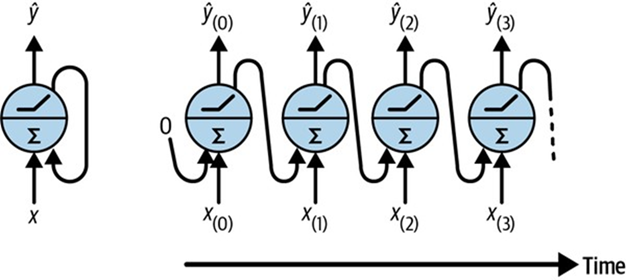
\includegraphics[width=\textwidth,height=0.65\textheight,keepaspectratio]{../machineLearningWeb/Figures/CH15/Hình_15-1.png}
            \vspace{0.2cm} \textit{Hình 15-1: RNN cơ bản và phiên bản mở rộng}
        \end{column}
    \end{columns}
\end{frame}

\begin{frame}{Trạng thái Ẩn (Hidden State) và Tính Toán Toán Học}
    \begin{itemize}
        \item Tại mỗi bước thời gian $t$, nơ-ron RNN (hoặc lớp RNN) tính toán trạng thái tiếp theo như sau:
        $$ \mathbf{h}_{(t)} = \phi \left( \mathbf{W}_{hx} \mathbf{x}_{(t)} + \mathbf{W}_{hh} \mathbf{h}_{(t-1)} + \mathbf{b} \right) $$
        \item Trong đó:
        \begin{itemize}
            \item $\mathbf{x}_{(t)}$: Đầu vào tại bước $t$.
            \item $\mathbf{h}_{(t-1)}$: Trạng thái ẩn từ bước $t-1$ (mang thông tin "trí nhớ").
            \item $\mathbf{W}_{hx}$: Trọng số cho đầu vào.
            \item $\mathbf{W}_{hh}$: Trọng số cho trạng thái ẩn.
            \item $\mathbf{b}$: Vector độ lệch (bias).
            \item $\phi$: Hàm kích hoạt (thường dùng \texttt{tanh} thay vì \texttt{ReLU} ở RNN chuẩn để tránh phát nổ giá trị).
        \end{itemize}
    \end{itemize}
\end{frame}

\begin{frame}{Đặc điểm của Trọng Số trong RNN}
    \begin{itemize}
        \item \textbf{Chia sẻ Trọng số (Weight Sharing):}
        \item Khác với mạng MLP nơi mỗi lớp có bộ trọng số riêng, RNN sử dụng \textbf{cùng một bộ ma trận trọng số $\mathbf{W}_{hx}, \mathbf{W}_{hh}$} cho tất cả các bước thời gian $t$.
        \item Lợi ích:
        \begin{itemize}
            \item Giảm số lượng tham số đáng kể, tránh quá khớp (overfitting).
            \item Có khả năng tổng quát hóa cho các chuỗi có độ dài chưa từng thấy trong tập huấn luyện.
        \end{itemize}
    \end{itemize}
\end{frame}

\begin{frame}{Lớp RNN (RNN Cell Layer)}
    \begin{columns}
        \begin{column}{0.5\textwidth}
            \begin{itemize}
                \item Hình 15-2 biểu diễn một \textbf{lớp nơ-ron RNN} (RNN Layer) thay vì chỉ một nơ-ron đơn.
                \item Thay vì nhận một đặc trưng, mạng nhận một vector đặc trưng $\mathbf{x}_{(t)}$.
                \item Lớp này trả về vector đầu ra $\mathbf{y}_{(t)}$ (thường chính là $\mathbf{h}_{(t)}$).
                \item Ký hiệu vector giúp mở rộng sang phép tính ma trận cho \textbf{Mini-batch} (nhiều chuỗi cùng lúc).
            \end{itemize}
        \end{column}
        \begin{column}{0.5\textwidth}
            \centering
            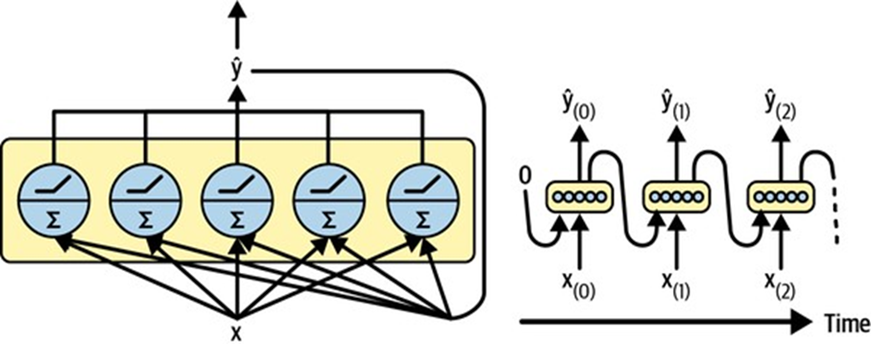
\includegraphics[width=\textwidth,height=0.65\textheight,keepaspectratio]{../machineLearningWeb/Figures/CH15/Hình_15-2.png}
            \vspace{0.2cm} \textit{Hình 15-2: Lớp RNN qua thời gian}
        \end{column}
    \end{columns}
\end{frame}

\section{2. Ứng dụng và Kiến Trúc Dựa Trên Chuỗi}

\begin{frame}{Phân loại Bài toán xử lý Chuỗi}
    Tùy thuộc vào yêu cầu đầu vào / đầu ra, ta có các loại bài toán:
    \vspace{0.5cm}
    \begin{enumerate}
        \item \textbf{Sequence-to-Sequence (Chuỗi sang Chuỗi đồng bộ):} Đầu vào $N$ bước, xuất $N$ bước. (Dự báo thời tiết liên tục).
        \item \textbf{Sequence-to-Vector (Chuỗi sang Vector):} Đầu vào $N$ bước, chỉ xuất 1 kết quả ở cuối chuỗi. (Phân loại văn bản, Sentiment analysis).
        \item \textbf{Vector-to-Sequence (Vector sang Chuỗi):} Đầu vào 1 giá trị, sinh ra chuỗi độ dài $N$. (Tạo chú thích ảnh - Image Captioning).
        \item \textbf{Encoder-Decoder (Delayed Seq-to-Seq):} Nhận chuỗi $N$, dịch qua chuỗi $M$. (Dịch máy, Trả lời câu hỏi).
    \end{enumerate}
\end{frame}

\begin{frame}{Minh Họa 4 Dạng Kiến Trúc RNN Cốt Lõi}
    \begin{columns}
        \begin{column}{0.4\textwidth}
            \textbf{Ghi chú Hình 15-4:} 
            \begin{itemize}
                \item \textit{Trên trái:} Seq-to-Seq (đồng bộ).
                \item \textit{Trên phải:} Seq-to-Vec. Đầu ra chỉ quan tâm ở bước cuối.
                \item \textit{Dưới trái:} Vec-to-Seq. Đầu vào duy nhất ở $t=0$.
                \item \textit{Dưới phải:} Mã hóa - Giải mã. Chờ hết câu rồi mới dịch.
            \end{itemize}
        \end{column}
        \begin{column}{0.6\textwidth}
            \centering
            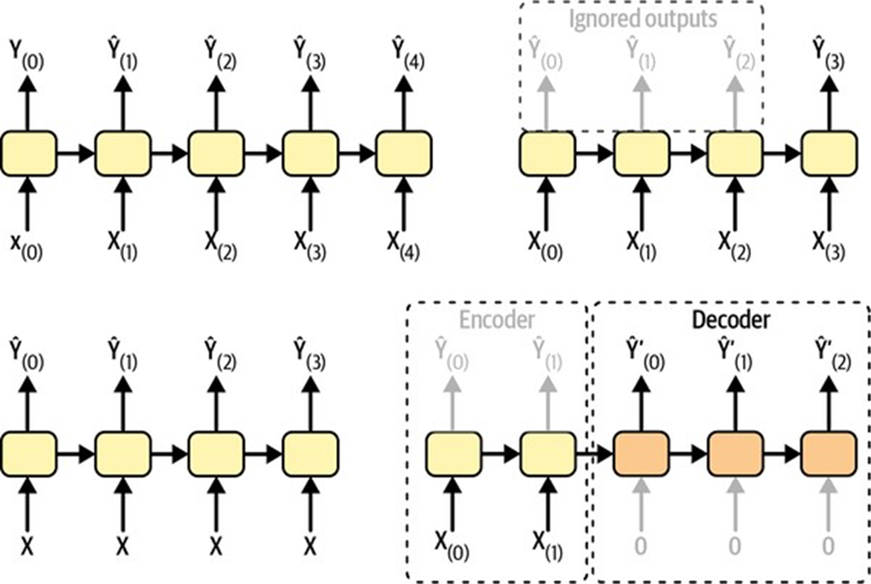
\includegraphics[width=\textwidth,height=0.75\textheight,keepaspectratio]{../machineLearningWeb/Figures/CH15/Hình_15-4.png}
            \vspace{0.2cm} \textit{Hình 15-4: Các dạng Seq2Seq, Seq2Vec, Vec2Seq}
        \end{column}
    \end{columns}
\end{frame}

\begin{frame}{Ứng Dụng: Mạng Chuỗi Sang Chuỗi Dự Báo Trễ}
    \begin{columns}
        \begin{column}{0.5\textwidth}
            \begin{itemize}
                \item \textbf{Hình 15-3} mô tả kiến trúc dùng nhiều nhất cho Time Series Forecasting (Dự báo chuỗi thời gian).
                \item Kỳ vọng mạng dự đoán tương lai $y_{(0)}, y_{(1)}...$ dựa trên quá khứ $x_{(0)}, x_{(1)},...$.
                \item Đầu ra $y_{(t)}$ tại thời điểm $t$ là kết quả dự báo cho $x_{(t+1)}$, do đó mạng bị trễ 1 bước (shifted by 1 step).
            \end{itemize}
        \end{column}
        \begin{column}{0.5\textwidth}
            \centering
            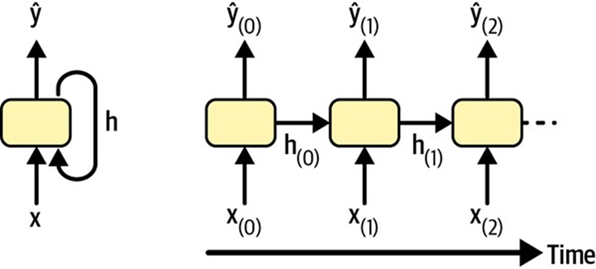
\includegraphics[width=\textwidth,height=0.65\textheight,keepaspectratio]{../machineLearningWeb/Figures/CH15/Hình_15-3.png}
            \vspace{0.2cm} \textit{Hình 15-3: Seq-to-Seq trễ trong dự báo}
        \end{column}
    \end{columns}
\end{frame}

\section{3. Huấn luyện RNN: BPTT}

\begin{frame}{Huấn luyện mạng Neural truyền thống (Nhắc lại)}
    \begin{itemize}
        \item Mạng truyền thẳng được huấn luyện bằng \textbf{Lan truyền ngược (Backpropagation)}:
        \begin{enumerate}
            \item Lan truyền xuôi (Forward pass) để tính hàm mất mát (Loss).
            \item Tính Gradient (đạo hàm) của Loss theo các trọng số từ lớp cuối về lớp đầu bằng quy tắc chuỗi (Chain rule).
            \item Cập nhật trọng số bằng Gradient Descent.
        \end{enumerate}
        \item Đối với RNN, chuỗi thời gian $t=1...T$ làm cấu trúc mạng giống như một mạng rất sâu $T$ lớp. Cần một biến thể đặc biệt.
    \end{itemize}
\end{frame}

\begin{frame}{Backpropagation Through Time (BPTT)}
    \begin{itemize}
        \item \textbf{Lan truyền ngược qua thời gian (BPTT)} là kỹ thuật huấn luyện RNN:
        \item \textbf{Bước 1 (Mở cuộn - Unrolling):} Tạm thời xem RNN như một mạng Feedforward khổng lồ với $T$ lớp (nếu chuỗi dài $T$).
        \item \textbf{Bước 2 (Lan truyền xuôi):} Tính Loss trên mọi bước thời gian (hoặc chỉ bước cuối).
        \item \textbf{Bước 3 (Lan truyền ngược):} Gradient lan truyền ngược dọc theo chiều thời gian từ $t=T$ về $t=0$.
        \item Tổng Gradient cho trọng số mạng là tổng của các Gradient tại mọi bước thời gian.
    \end{itemize}
\end{frame}

\begin{frame}{Cơ chế Hoạt động của BPTT (Minh họa)}
    \begin{columns}
        \begin{column}{0.5\textwidth}
            \begin{itemize}
                \item \textbf{Hình 15-5} minh họa quá trình BPTT.
                \item Mũi tên liền nét dày mô tả luồng Gradient ngược từ hàm mất mát $L$.
                \item Do $\mathbf{W}$ được chia sẻ ở mọi $t$, gradient cuối cùng để cập nhật $\mathbf{W}$ là tổng $\sum \nabla \mathbf{W}^{(t)}$.
                \item Phép tính này cực kỳ đắt đỏ và tốn RAM nếu độ dài chuỗi rất lớn.
            \end{itemize}
        \end{column}
        \begin{column}{0.5\textwidth}
            \centering
            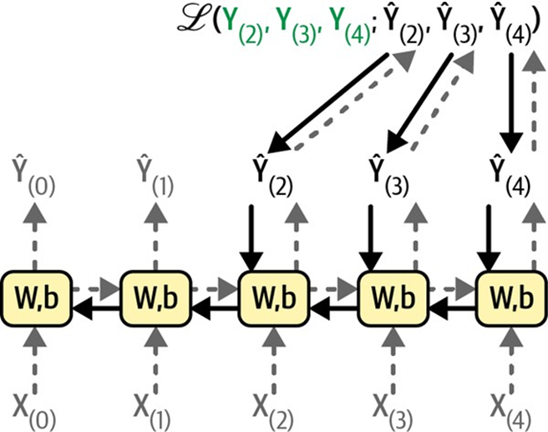
\includegraphics[width=\textwidth,height=0.7\textheight,keepaspectratio]{../machineLearningWeb/Figures/CH15/Hình_15-5.png}
            \vspace{0.2cm} \textit{Hình 15-5: BPTT - Lan truyền ngược qua thời gian}
        \end{column}
    \end{columns}
\end{frame}

\begin{frame}{Vấn Đề: Vanishing Gradients (Suy thoái Gradient)}
    \begin{itemize}
        \item \textbf{Nguyên nhân:} Trong BPTT, đạo hàm phải được nhân với ma trận trọng số $W_{hh}$ liên tục $T$ lần (qua $T$ bước thời gian).
        \item $\nabla h_{(0)} \propto (W_{hh})^T \nabla h_{(T)}$
        \item Nếu giá trị riêng lớn nhất của $W_{hh} < 1$, gradient tiến dần về $0$ theo hàm số mũ.
        \item \textbf{Hậu quả:} Mạng không thể học được phụ thuộc xa (Ví dụ: Từ ở đầu câu văn quá dài không có ảnh hưởng gì tới dự đoán ở cuối câu). Trí nhớ mạng bị "ngắn hạn".
    \end{itemize}
\end{frame}

\begin{frame}{Vấn Đề: Exploding Gradients (Bùng nổ Gradient)}
    \begin{itemize}
        \item Ngược lại, nếu giá trị riêng lớn nhất của $W_{hh} > 1$, gradient bị nhân lên theo cấp số nhân và phát nổ thành $NaN$ hoặc vô cực.
        \item \textbf{Hậu quả:} Cập nhật trọng số quá lớn, làm mất ổn định hoàn toàn mạng, Loss dao động điên cuồng.
        \item \textbf{Giải pháp cho bùng nổ:}
        \begin{itemize}
            \item \textbf{Gradient Clipping:} Cắt cụt gradient nếu nó vượt quá một ngưỡng nhất định trước khi cập nhật.
            \item Thường xuyên được áp dụng mặc định trong các Framework như Keras/PyTorch.
        \end{itemize}
    \end{itemize}
\end{frame}

\section{4. Dự báo Chuỗi Thời Gian (Time Series)}

\begin{frame}{Bài toán Dự báo Chuỗi Thời Gian Thực Tế}
    \begin{itemize}
        \item Chúng ta sẽ xem xét dữ liệu thực tế để hiểu tại sao cần RNN phức tạp.
        \item Dự báo chuỗi thời gian (Time series forecasting) thường phải xử lý:
        \begin{itemize}
            \item Nhiễu trắng (White noise) ngẫu nhiên.
            \item Tính thời vụ (Seasonality) - Các mẫu lặp lại đặn (Ngày, tuần, tháng).
            \item Xu hướng (Trend) - Tăng trưởng hoặc suy giảm chậm trong thời gian dài.
        \end{itemize}
        \item Tiền xử lý dữ liệu để loại bỏ những yếu tố này đôi khi hiệu quả hơn để mạng nơ-ron tự học từ đầu.
    \end{itemize}
\end{frame}

\begin{frame}{Ví dụ: Lượng hành khách xe buýt (Chicago)}
    \begin{columns}
        \begin{column}{0.4\textwidth}
            \begin{itemize}
                \item Tập dữ liệu lượng hành khách hàng ngày ở Chicago (2019).
                \item Trục hoành là Ngày, trục tung là số hành khách.
                \item \textbf{Hình 15-6} cho thấy các biến động liên tục và nhịp nhàng. Mỗi "khối" lởm chởm tương ứng với một tuần làm việc (cao điểm) và cuối tuần (giảm sút).
            \end{itemize}
        \end{column}
        \begin{column}{0.6\textwidth}
            \centering
            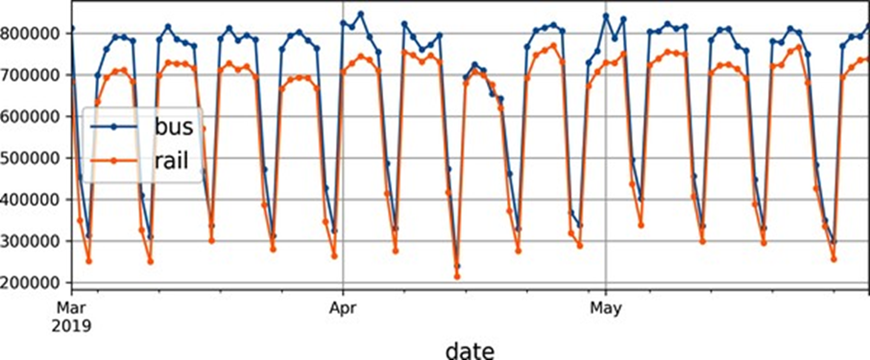
\includegraphics[width=\textwidth,height=0.65\textheight,keepaspectratio]{../machineLearningWeb/Figures/CH15/Hình_15-6.png}
            \vspace{0.2cm} \textit{Hình 15-6: Lượng hành khách hằng ngày ở Chicago}
        \end{column}
    \end{columns}
\end{frame}

\begin{frame}{Kỹ thuật Tiền Xử Lý: Sai phân (Differencing)}
    \begin{columns}
        \begin{column}{0.5\textwidth}
            \begin{itemize}
                \item Để giúp mạng dễ dàng học hơn, ta có thể khử \textbf{tính thời vụ hàng tuần} bằng phép tính sai phân trễ 7 ngày ($y_t - y_{t-7}$).
                \item \textbf{Hình 15-7} cho thấy: Biểu đồ trên mô tả chuỗi gốc so với chuỗi bị dịch (trễ).
                \item Biểu đồ dưới (chuỗi sai phân) mượt mà, stationary (dừng) và loại bỏ được nhiễu do khác biệt giữa ngày thường và cuối tuần.
            \end{itemize}
        \end{column}
        \begin{column}{0.5\textwidth}
            \centering
            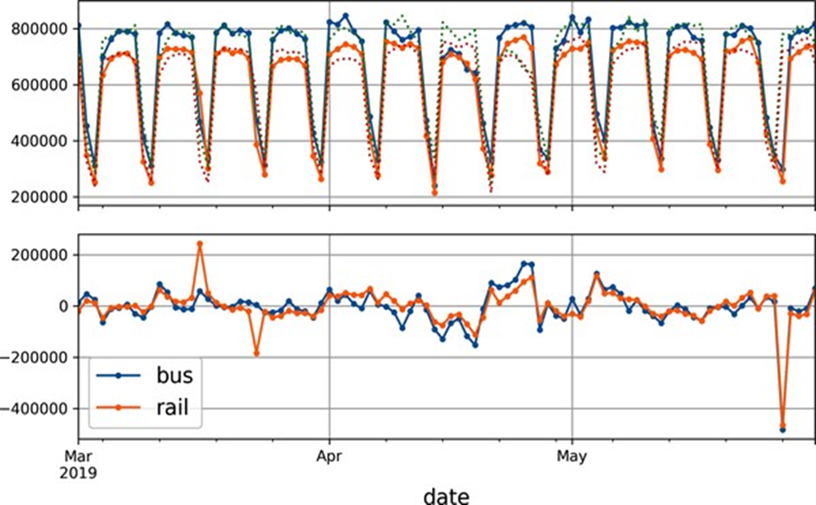
\includegraphics[width=\textwidth,height=0.7\textheight,keepaspectratio]{../machineLearningWeb/Figures/CH15/Hình_15-7.png}
            \vspace{0.2cm} \textit{Hình 15-7: Chuỗi thời gian trễ 7 ngày và phép sai phân}
        \end{column}
    \end{columns}
\end{frame}

\begin{frame}{Kỹ thuật Tiền Xử Lý: Xu Hướng Vĩ Mô}
    \begin{columns}
        \begin{column}{0.5\textwidth}
            \begin{itemize}
                \item Mở rộng ra 15 năm (2001-2015), \textbf{Hình 15-8} cho thấy rõ ràng các ngày lễ hội khiến lượng khách sụt giảm lớn hàng năm, và tổng thể hành khách biến động vĩ mô (Macro Trend).
                \item Để RNN mô hình hóa được điều này, nó cần "Trí nhớ Dài Hạn" vươn xa hàng trăm bước, cực kỳ khó nếu dùng \texttt{SimpleRNN}.
            \end{itemize}
        \end{column}
        \begin{column}{0.5\textwidth}
            \centering
            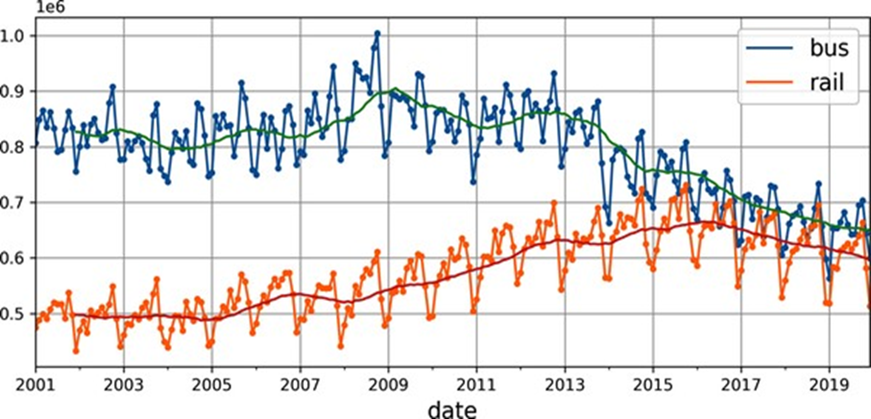
\includegraphics[width=\textwidth,height=0.7\textheight,keepaspectratio]{../machineLearningWeb/Figures/CH15/Hình_15-8.png}
            \vspace{0.2cm} \textit{Hình 15-8: Tính thời vụ hằng năm và xu hướng dài hạn}
        \end{column}
    \end{columns}
\end{frame}

\begin{frame}{Kỹ thuật Tiền Xử Lý: Sai phân Dài hạn}
    \begin{columns}
        \begin{column}{0.45\textwidth}
            \begin{itemize}
                \item Áp dụng sai phân 12 tháng liên tục.
                \item \textbf{Hình 15-9} cho thấy chuỗi kết quả cân bằng hơn quanh mốc 0.
                \item Mạng RNN hiện đại có thể tự phát hiện các trend này, nhưng trong thực tế, đưa vào chuỗi sai phân thường hội tụ nhanh và dự đoán chính xác hơn dữ liệu gốc hỗn độn.
            \end{itemize}
        \end{column}
        \begin{column}{0.55\textwidth}
            \centering
            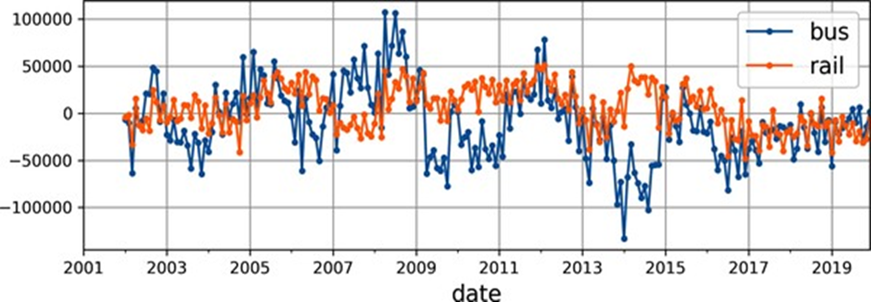
\includegraphics[width=\textwidth,height=0.65\textheight,keepaspectratio]{../machineLearningWeb/Figures/CH15/Hình_15-9.png}
            \vspace{0.2cm} \textit{Hình 15-9: Sự sai phân 12 tháng (Dài hạn)}
        \end{column}
    \end{columns}
\end{frame}

\begin{frame}[fragile]{Code: API Huấn luyện RNN cơ bản với Keras}
    Để xây dựng \texttt{SimpleRNN} trên Keras, dùng lớp mô phỏng nơ-ron hồi quy:
\begin{lstlisting}[language=Python]
import tensorflow as tf
from tensorflow import keras

# Tao mang RNN 1 lop, 1 hidden unit
model = keras.Sequential([
    keras.layers.SimpleRNN(1, input_shape=[None, 1])
])

model.compile(loss="mse", optimizer="adam")
history = model.fit(X_train, y_train, epochs=20,
                    validation_data=(X_valid, y_valid))
\end{lstlisting}
\end{frame}

\begin{frame}{Phân tích Code Keras RNN}
    \begin{itemize}
        \item Tham số \texttt{1} trong \texttt{SimpleRNN(1)} là số lượng nơ-ron trạng thái ẩn (dimensionality of output space). Vì là dự đoán 1 bước tiếp theo (đại lượng vô hướng), nên chọn 1 nơ-ron.
        \item \texttt{input\_shape=[None, 1]}:
        \begin{itemize}
            \item \texttt{None}: Đại diện cho chiều dài của chuỗi (Time steps). Keras cho phép chuỗi dài ngắn tùy ý nếu ta đặt là None.
            \item \texttt{1}: Số chiều (Features) tại mỗi bước thời gian. (Chỉ có 1 đặc trưng là lượng hành khách).
        \end{itemize}
        \item Hàm Loss thường dùng cho bài toán dự báo chuỗi là Mean Squared Error (\texttt{mse}) hoặc Mean Absolute Error (\texttt{mae}).
    \end{itemize}
\end{frame}

\section{5. Mạng RNN Sâu (Deep RNNs)}

\begin{frame}{Kiến trúc Mạng RNN Sâu}
    \begin{columns}
        \begin{column}{0.5\textwidth}
            \begin{itemize}
                \item Tương tự MLP Sâu, ta \textbf{xếp chồng (stacking)} các lớp RNN lên nhau tạo thành \textbf{Deep RNN}.
                \item Lớp dưới cùng nhận dữ liệu đầu vào. Đầu ra trạng thái ẩn $\mathbf{h}_{(t)}$ của lớp dưới làm đầu vào cho lớp trên tại \textbf{cùng thời điểm} $t$.
                \item \textbf{Hình 15-10} chỉ ra mũi tên lan truyền dọc theo cả 2 trục: Trục thời gian (ngang) và Trục không gian / Chiều sâu (dọc).
            \end{itemize}
        \end{column}
        \begin{column}{0.5\textwidth}
            \centering
            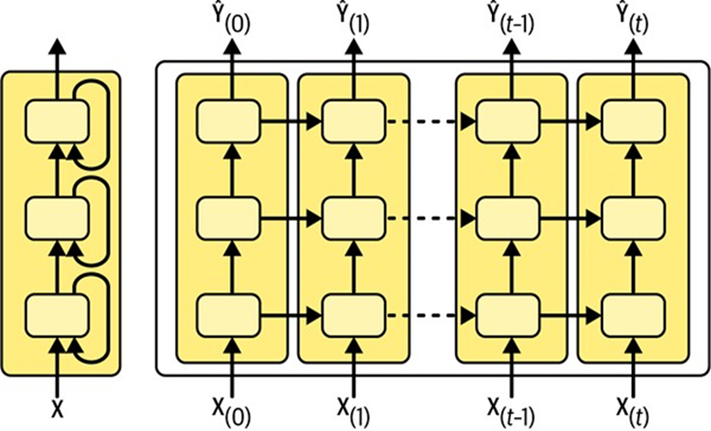
\includegraphics[width=\textwidth,height=0.7\textheight,keepaspectratio]{../machineLearningWeb/Figures/CH15/Hình_15-10.png}
            \vspace{0.2cm} \textit{Hình 15-10: Mạng RNN sâu nhiều lớp}
        \end{column}
    \end{columns}
\end{frame}

\begin{frame}[fragile]{Code: Xây dựng Mạng RNN Sâu}
    \begin{itemize}
        \item Yêu cầu quan trọng: Để lớp RNN dưới có thể đẩy chuỗi output lên lớp RNN trên, nó BẮT BUỘC phải bật \texttt{return\_sequences=True}.
    \end{itemize}
\begin{lstlisting}[language=Python]
deep_model = keras.Sequential([
    # Lop RNN 1: Tra ve chuoi cho lop 2
    keras.layers.SimpleRNN(20, return_sequences=True, input_shape=[None, 1]),
    # Lop RNN 2: Tra ve chuoi cho lop cuoi
    keras.layers.SimpleRNN(20, return_sequences=True),
    # Lop RNN cuoi: Chi tra ve vector cuoi cung (Seq2Vec)
    keras.layers.SimpleRNN(1) 
])
\end{lstlisting}
\end{frame}

\begin{frame}{Dự báo nhiều bước (Multi-step Forecasting)}
    \begin{itemize}
        \item Mạng trên chỉ dự báo $t+1$. Để dự báo xa (VD: $t+10$), có 2 cách:
        \begin{enumerate}
            \item \textbf{Cách 1 (Dự đoán tuần tự - Autoregressive):} Dự đoán $t+1$, lấy giá trị đó gộp vào mảng đầu vào để đoán $t+2$, lặp lại 10 lần. (Dễ tích lũy sai số).
            \item \textbf{Cách 2 (Dự đoán đồng thời):} Đổi lớp cuối thành \texttt{Dense(10)} để bắt mạng xuất 10 giá trị cùng một lúc. Cách này thường ổn định hơn.
        \end{enumerate}
    \end{itemize}
\end{frame}

\begin{frame}{Kết quả dự báo đa bước của RNN Sâu}
    \begin{columns}
        \begin{column}{0.4\textwidth}
            \begin{itemize}
                \item \textbf{Hình 15-11} là kết quả dự báo một chuỗi nhân tạo nhiều bước đồng thời.
                \item Dấu \texttimes{} là dữ liệu đầu vào.
                \item Đường đứt nét là giá trị mục tiêu (Target).
                \item Dấu chấm tròn là giá trị dự đoán do mạng RNN sâu đưa ra.
                \item Mạng bám sát rất tốt đường đi tự nhiên của sóng dốc.
            \end{itemize}
        \end{column}
        \begin{column}{0.6\textwidth}
            \centering
            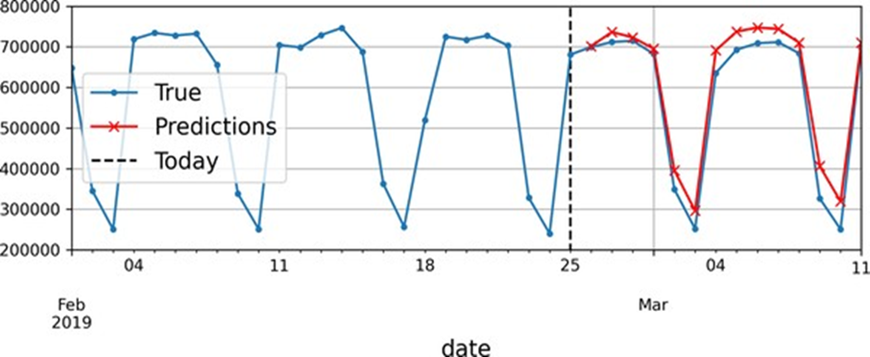
\includegraphics[width=\textwidth,height=0.7\textheight,keepaspectratio]{../machineLearningWeb/Figures/CH15/Hình_15-11.png}
            \vspace{0.2cm} \textit{Hình 15-11: RNN Sâu dự báo đa bước khá chính xác}
        \end{column}
    \end{columns}
\end{frame}

\section{6. Kiến trúc Tế bào Nhớ: LSTM và GRU}

\begin{frame}{Vấn đề cốt lõi của SimpleRNN (Nhắc lại)}
    \begin{itemize}
        \item SimpleRNN rất tồi trong việc nắm bắt \textbf{phụ thuộc xa (Long-Term Dependencies)}.
        \item Ví dụ câu NLP: \textit{"Tôi sống ở Pháp từ nhỏ, sau 20 năm chuyển đến Mỹ, tôi vẫn nói trôi chảy tiếng [X]."}. Mạng cần nhớ chữ \textit{"Pháp"} ở quá khứ rất xa để đoán chữ \textit{"Pháp"}.
        \item Trọng số $W$ nếu nhỏ thì Vanishing Gradient làm chữ "Pháp" bốc hơi sau vài bước thời gian.
        \item Để tạo ra "Trí nhớ Dài hạn", \textbf{Tế bào LSTM} được phát minh (Hochreiter và Schmidhuber - 1997).
    \end{itemize}
\end{frame}

\begin{frame}{Sơ lược về Tế bào LSTM (Long Short-Term Memory)}
    \begin{itemize}
        \item Ý tưởng cốt lõi của LSTM là thay vì chỉ truyền một Trạng thái ẩn $h_{(t)}$, nó duy trì thêm một đường truyền phụ gọi là \textbf{Trạng thái tế bào (Cell State - $c_{(t)}$)}.
        \item $c_{(t)}$ giống như một đường ray cao tốc, chạy dọc xuyên suốt quá trình thời gian, cho phép thông tin truyền đi rất xa mà không suy giảm.
        \item Các cơ chế điều tiết (Gates - Cổng) kiểm soát việc ghi, đọc, xóa dữ liệu trên đường ray $c_{(t)}$ này.
    \end{itemize}
\end{frame}

\begin{frame}{Cấu trúc Tế bào LSTM chi tiết}
    \begin{columns}
        \begin{column}{0.45\textwidth}
            \begin{itemize}
                \item \textbf{Hình 15-12} là mô hình LSTM chuẩn. Đường ray ngang ở trên cùng là Trạng thái tế bào $c_{(t)}$. Đường ray dưới là Trạng thái ẩn $h_{(t)}$.
                \item Các phép toán tròn như $\otimes, \oplus$ là phép nhân phần tử và phép cộng vector.
                \item Cổng (Gate) sử dụng hàm kích hoạt Sigmoid ($\sigma$) (xuất giá trị [0, 1]) hoạt động như một cái "van": 0 là đóng hoàn toàn, 1 là mở hoàn toàn.
            \end{itemize}
        \end{column}
        \begin{column}{0.55\textwidth}
            \centering
            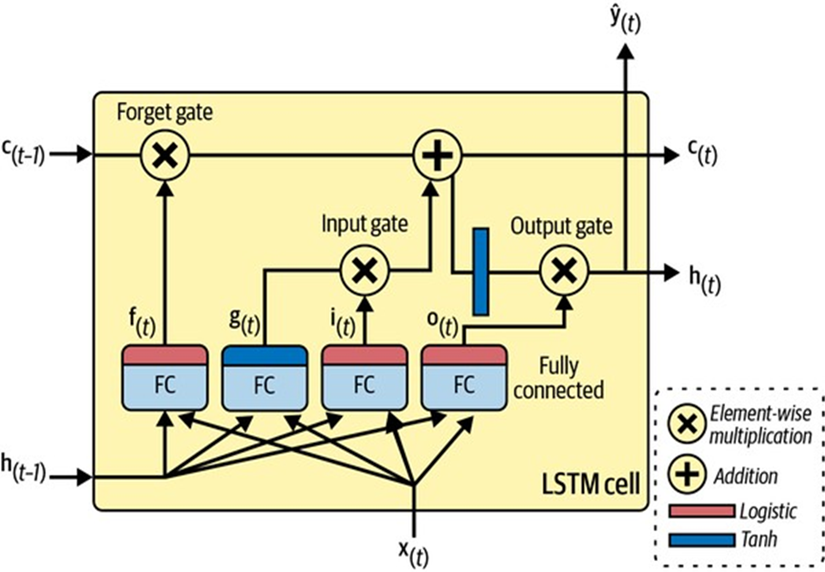
\includegraphics[width=\textwidth,height=0.7\textheight,keepaspectratio]{../machineLearningWeb/Figures/CH15/Hình_15-12.png}
            \vspace{0.2cm} \textit{Hình 15-12: Cấu tạo bên trong Tế bào LSTM}
        \end{column}
    \end{columns}
\end{frame}

\begin{frame}{Phân tích 3 Cổng của LSTM (Phần 1)}
    Dựa vào sơ đồ \textbf{Hình 15-12}:
    \begin{itemize}
        \item \textbf{1. Cổng Quên (Forget Gate - $f_{(t)}$):} 
        \begin{itemize}
            \item Nhận vào $h_{(t-1)}$ và $x_{(t)}$, tính toán bằng Sigmoid.
            \item Quyết định phần nào của Trạng thái dài hạn $c_{(t-1)}$ sẽ bị "bỏ đi". (Ví dụ: Thấy chủ ngữ mới thì quên chủ ngữ cũ).
        \end{itemize}
        \item \textbf{2. Cổng Cập nhật \& Ghi (Input Gate - $i_{(t)}, g_{(t)}$):}
        \begin{itemize}
            \item $g_{(t)}$ tạo ra một vector giá trị ứng viên mới (dùng $\tanh$).
            \item $i_{(t)}$ quyết định (bằng Sigmoid) mức độ quan trọng của các ứng viên này để cộng vào $c_{(t)}$ làm thông tin mới.
        \end{itemize}
    \end{itemize}
\end{frame}

\begin{frame}{Phân tích 3 Cổng của LSTM (Phần 2)}
    \begin{itemize}
        \item \textbf{Cập nhật Trạng thái Tế bào ($c_{(t)}$):}
        $$ c_{(t)} = f_{(t)} \otimes c_{(t-1)} + i_{(t)} \otimes g_{(t)} $$
        (Quên đi quá khứ không cần thiết + Nhớ thêm thông tin mới).
        \vspace{0.5cm}
        \item \textbf{3. Cổng Xuất (Output Gate - $o_{(t)}$):}
        \begin{itemize}
            \item Quyết định phần nào của Trạng thái Tế bào $c_{(t)}$ sẽ được đọc ra và đưa vào Trạng thái ẩn $h_{(t)}$.
            \item $o_{(t)} = \sigma(W_o [x_{(t)}, h_{(t-1)}])$
            \item $h_{(t)} = o_{(t)} \otimes \tanh(c_{(t)})$
        \end{itemize}
    \end{itemize}
\end{frame}

\begin{frame}[fragile]{Sử dụng LSTM trong Keras}
    \begin{itemize}
        \item Cực kỳ đơn giản, chỉ cần thay \texttt{SimpleRNN} bằng \texttt{LSTM}. Mọi công thức cổng phức tạp bên trên đã được Keras tối ưu bằng thư viện CUDNN dưới nền.
    \end{itemize}
\begin{lstlisting}[language=Python]
model = keras.Sequential([
    keras.layers.LSTM(20, return_sequences=True, input_shape=[None, 1]),
    keras.layers.LSTM(20),
    keras.layers.Dense(1)
])
\end{lstlisting}
    \begin{itemize}
        \item LSTM giải quyết tốt chuỗi dài khoảng hàng trăm bước thời gian, vượt xa SimpleRNN (chỉ hiệu quả với < 20 bước).
    \end{itemize}
\end{frame}

\begin{frame}{Tế bào GRU (Gated Recurrent Unit)}
    \begin{columns}
        \begin{column}{0.5\textwidth}
            \begin{itemize}
                \item GRU (2014) là một nỗ lực đơn giản hóa cấu trúc của LSTM.
                \item Hai điểm khác biệt chính:
                \begin{enumerate}
                    \item GRU không có đường ray $c_{(t)}$ riêng biệt. Nó gộp chung Trạng thái ẩn $h_{(t)}$ và Trạng thái tế bào làm một.
                    \item Gộp Cổng Quên và Cổng Cập nhật thành một \textbf{Cổng Cập nhật (Update Gate - $z_{(t)}$)}. Nếu $z=1$ thì lưu mới, nếu $z=0$ thì giữ cũ.
                \end{enumerate}
            \end{itemize}
        \end{column}
        \begin{column}{0.5\textwidth}
            \centering
            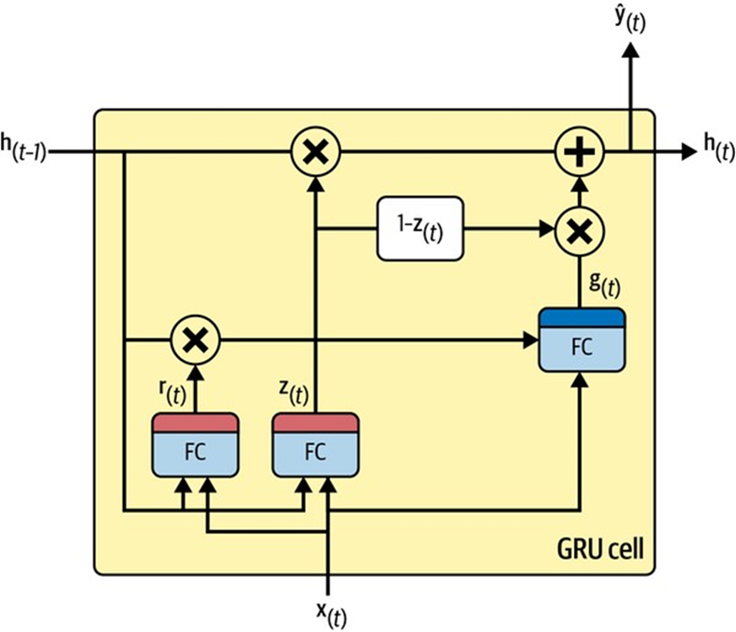
\includegraphics[width=\textwidth,height=0.8\textheight,keepaspectratio]{../machineLearningWeb/Figures/CH15/Hình_15-13.png}
            \vspace{0.2cm} \textit{Hình 15-13: Cấu tạo Tế bào GRU}
        \end{column}
    \end{columns}
\end{frame}

\begin{frame}{So sánh LSTM và GRU}
    \begin{table}[]
        \centering
        \begin{tabular}{|l|c|c|}
            \hline
            \textbf{Đặc điểm} & \textbf{LSTM} & \textbf{GRU} \\ \hline
            Năm ra đời & 1997 & 2014 \\ \hline
            Trạng thái duy trì & $h_t$ và $c_t$ & Chỉ $h_t$ \\ \hline
            Số lượng Cổng & 3 (Quên, Nhập, Xuất) & 2 (Cập nhật, Reset) \\ \hline
            Tốc độ huấn luyện & Chậm & Nhanh hơn \\ \hline
            Số lượng tham số & Lớn (Nặng RAM) & Thấp hơn ($\sim 25\%$ ít hơn) \\ \hline
            Độ chính xác & Tốt với chuỗi rất phức tạp & Ngang ngửa LSTM ở đa số Data \\ \hline
        \end{tabular}
    \end{table}
    \begin{itemize}
        \item \textbf{Lời khuyên thực tiễn:} Bắt đầu thử nghiệm với GRU vì nó nhanh. Nếu thấy hiệu năng có vẻ bị thắt nút, chuyển sang LSTM xem có cải thiện không.
    \end{itemize}
\end{frame}

\section{7. WaveNet (Mạng CNN 1D cho Chuỗi)}

\begin{frame}{Tại sao lại dùng CNN cho Dữ liệu Chuỗi?}
    \begin{itemize}
        \item RNN (ngay cả LSTM/GRU) có một điểm yếu chết người: \textbf{Tính toán tuần tự}.
        \item Bạn không thể tính bước thời gian $t=100$ nếu chưa tính xong bước $t=99$. Điều này khiến RNN \textbf{không thể chạy song song} trên phần cứng GPU một cách hiệu quả.
        \item Mạng Tích chập (CNN) với Kernel trượt thì độc lập với nhau, \textbf{hoàn toàn song song hóa} được.
        \item Ta có thể dùng \textbf{CNN 1D} (chỉ quét theo chiều dài thời gian) để trích xuất đặc trưng chuỗi.
    \end{itemize}
\end{frame}

\begin{frame}{Hạn chế của CNN 1D truyền thống}
    \begin{itemize}
        \item Bộ lọc (Kernel) CNN 1D có kích thước nhỏ (VD: size 3).
        \item Nghĩa là mỗi nơ-ron lớp CNN 1 chỉ nhìn thấy 3 bước thời gian.
        \item Để nhìn được 100 bước thời gian (Trường thụ cảm - Receptive field lớn), ta phải xếp chồng hàng chục lớp CNN 1D, kết hợp với các lớp Pooling.
        \item Việc này rất nặng nề và làm mất đi thông tin chuỗi chi tiết. Cần một cơ chế quét khác!
    \end{itemize}
\end{frame}

\begin{frame}{Giải pháp đột phá: Kiến trúc WaveNet (2016)}
    \begin{columns}
        \begin{column}{0.4\textwidth}
            \begin{itemize}
                \item WaveNet do DeepMind phát triển, chuyên tạo giọng nói Audio. Âm thanh có tới 16,000 mẫu/giây $\Rightarrow$ Chuỗi cực kỳ dài!
                \item Thay vì CNN thường, nó sử dụng \textbf{Tích chập giãn nở (Dilated Convolutions)}.
                \item \textbf{Hình 15-14} minh họa: Tỷ lệ giãn (Dilation rate) tăng dần theo lũy thừa $2^n$ (1, 2, 4, 8...).
            \end{itemize}
        \end{column}
        \begin{column}{0.6\textwidth}
            \centering
            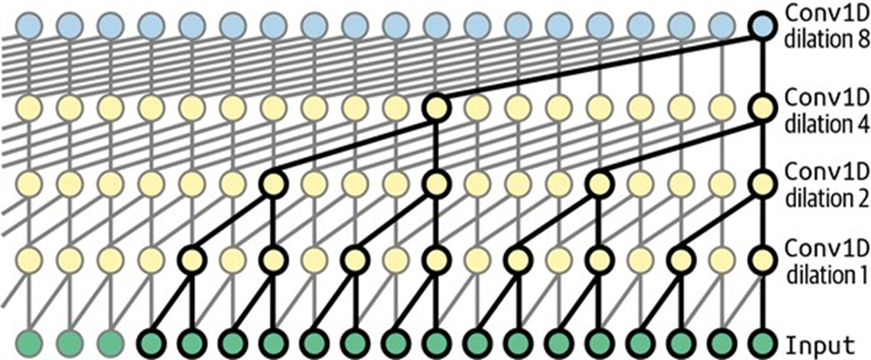
\includegraphics[width=\textwidth,height=0.85\textheight,keepaspectratio]{../machineLearningWeb/Figures/CH15/Hình_15-14.png}
            \vspace{0.2cm} \textit{Hình 15-14: Kiến trúc WaveNet (Dilated Conv)}
        \end{column}
    \end{columns}
\end{frame}

\begin{frame}{Cách hoạt động của Dilated Convolution}
    \begin{itemize}
        \item Lớp 1 (rate=1): Kernel trượt từng ô liền kề (Giống hệt Conv1D thường).
        \item Lớp 2 (rate=2): Kernel bỏ qua 1 ô xen kẽ, giúp 1 nơ-ron bao phủ được khoảng cách 4 ô.
        \item Lớp 3 (rate=4): Kernel bỏ qua 3 ô xen kẽ, một nơ-ron nhìn được 8 ô.
        \item Nhờ tăng rate theo lũy thừa, mạng chỉ cần 10 lớp là đã có Trường thụ cảm bao phủ được \textbf{1024 bước thời gian} mà số lượng tham số vẫn cực kỳ nhỏ.
    \end{itemize}
\end{frame}

\begin{frame}[fragile]{Code: Xây dựng WaveNet với Keras}
    Ta dùng vòng lặp để tạo các lớp \texttt{Conv1D} giãn nở:
\begin{lstlisting}[language=Python]
model = keras.Sequential()
model.add(keras.layers.InputLayer(input_shape=[None, 1]))

# Cac lop tich chap gian no (1, 2, 4, 8) lap lai
for rate in (1, 2, 4, 8) * 2:
    model.add(keras.layers.Conv1D(
        filters=20, kernel_size=2, padding="causal",
        activation="relu", dilation_rate=rate))

model.add(keras.layers.Conv1D(filters=10, kernel_size=1))
model.add(keras.layers.Dense(1)) # Lop du doan
\end{lstlisting}
    \begin{itemize}
        \item Tham số \texttt{padding="causal"} cực kỳ quan trọng ở Time Series, nó chèn 0 vào bên trái để Kernel không bao giờ với tới thông tin của "tương lai".
    \end{itemize}
\end{frame}

\section{Tổng kết}

\begin{frame}{Tổng Kết Chương 15 (Phần 1)}
    \begin{itemize}
        \item \textbf{Sequence Data:} Đòi hỏi mô hình có bộ nhớ để theo dõi thứ tự.
        \item \textbf{RNN Cơ bản:} Chia sẻ trọng số qua các bước thời gian. Dùng Trạng thái ẩn $h_{(t)}$ để mang thông tin tới tương lai.
        \item \textbf{Ứng dụng RNN đa dạng:} Seq2Seq (Dự báo, Dịch), Seq2Vec (Phân tích cảm xúc), Encoder-Decoder (Chatbot).
        \item \textbf{BPTT (Backpropagation Through Time):} Mở cuộn mạng qua không gian thời gian. Dễ gây ra hiện tượng Gradient bốc hơi hoặc bùng nổ khi chuỗi quá dài.
    \end{itemize}
\end{frame}

\begin{frame}{Tổng Kết Chương 15 (Phần 2)}
    \begin{itemize}
        \item \textbf{Tiền xử lý chuỗi (Differencing):} Rất hữu ích để loại bỏ tính thời vụ và xu hướng trước khi đưa vào mạng học sâu.
        \item \textbf{LSTM \& GRU:} Thiết kế Tế bào thông minh với các "Cổng" (Gate) động đóng mở bằng Sigmoid, giúp bảo toàn Gradient đi xa, mang lại "Trí nhớ Dài Hạn".
        \item \textbf{CNN 1D \& WaveNet:} Một hướng đi song song (không tuần tự), nhanh hơn RNN, dùng Dilated Convolutions để nắm bắt chuỗi độ dài hàng chục ngàn bước (vd: Âm thanh).
    \end{itemize}
\end{frame}

\end{document}
